\documentclass[bachelor, och, otchet]{SCWorks}
% Тип обучения (одно из значений):
%    bachelor   - бакалавриат (по умолчанию)
%    spec       - специальность
%    master     - магистратура
% Форма обучения (одно из значений):
%    och        - очное (по умолчанию)
%    zaoch      - заочное
% Тип работы (одно из значений):
%    coursework - курсовая работа (по умолчанию)
%    referat    - реферат
%  * otchet     - универсальный отчет
%  * nirjournal - журнал НИР
%  * digital    - итоговая работа для цифровой кафедры
%    diploma    - дипломная работа
%    pract      - отчет о научно-исследовательской работе
%    autoref    - автореферат выпускной работы
%    assignment - задание на выпускную квалификационную работу
%    review     - отзыв руководителя
%    critique   - рецензия на выпускную работу

% * Добавлены вручную. За вопросами к @mchernigin
\usepackage{preamble}

\begin{document}

% Кафедра (в родительном падеже)
\chair{информатики и программирования}

% Тема работы
\title{Машинно"=зависимые языки программмирования. Лабораторная работа №2}

% Курс
\course{2}

% Группа
\group{251}

% Факультет (в родительном падеже) (по умолчанию "факультета КНиИТ")
\department{факультета компьютерных наук и информационных технологий}

% Специальность/направление код - наименование
% \napravlenie{02.03.02 "--- Фундаментальная информатика и информационные технологии}
% \napravlenie{02.03.01 "--- Математическое обеспечение и администрирование информационных систем}
% \napravlenie{09.03.01 "--- Информатика и вычислительная техника}
\napravlenie{09.03.04 "--- Программная инженерия}
% \napravlenie{10.05.01 "--- Компьютерная безопасность}

% Для студентки. Для работы студента следующая команда не нужна.
\studenttitle{студентки}

% Фамилия, имя, отчество в родительном падеже
\author{Потапкиной Маргариты Андреевны}

% Заведующий кафедрой 
\chtitle{доцент, к.\,ф.-м.\,н.}
\chname{С.\,В.\,Миронов}

% Руководитель ДПП ПП для цифровой кафедры (перекрывает заведующего кафедры)
% \chpretitle{
%     заведующий кафедрой математических основ информатики и олимпиадного\\
%     программирования на базе МАОУ <<Ф"=Т лицей №1>>
% }
% \chtitle{г. Саратов, к.\,ф.-м.\,н., доцент}
% \chname{Кондратова\, Ю.\,Н.}

% Научный руководитель (для реферата преподаватель проверяющий работу)
\satitle{старший преподаватель} %должность, степень, звание
\saname{Е.\,М.\,Черноусова}

% Руководитель практики от организации (руководитель для цифровой кафедры)
\patitle{доцент, к.\,ф.-м.\,н.}
\paname{С.\,В.\,Миронов}

% Руководитель НИР
\nirtitle{доцент, к.\,п.\,н.} % степень, звание
\nirname{В.\,А.\,Векслер}

% Семестр (только для практики, для остальных типов работ не используется)
\term{2}

% Наименование практики (только для практики, для остальных типов работ не
% используется)
\practtype{учебная}

% Продолжительность практики (количество недель) (только для практики, для
% остальных типов работ не используется)
\duration{2}

% Даты начала и окончания практики (только для практики, для остальных типов
% работ не используется)
\practStart{01.07.2024}
\practFinish{13.01.2024}

% Год выполнения отчета
\date{2025}

\maketitle

% Включение нумерации рисунков, формул и таблиц по разделам (по умолчанию -
% нумерация сквозная) (допускается оба вида нумерации)
\secNumbering

\tableofcontents

% Раздел "Обозначения и сокращения". Может отсутствовать в работе
% \abbreviations
% \begin{description}
%     \item ... "--- ...
%     \item ... "--- ...
% \end{description}

% Раздел "Определения". Может отсутствовать в работе
% \definitions

% Раздел "Определения, обозначения и сокращения". Может отсутствовать в работе.
% Если присутствует, то заменяет собой разделы "Обозначения и сокращения" и
% "Определения"
% \defabbr

\section{Текст задания}
\input{task.txt}

\section{Тексты программ на языке ассемблера с комментариями}
\subsection{Программа 1}
\small
\inputminted{nasm}{4.asm}
\subsection{Программа 2}
\inputminted{nasm}{5.asm}
\normalsize

\section{Скриншоты запуска программ}
\begin{figure}[H]
\centering
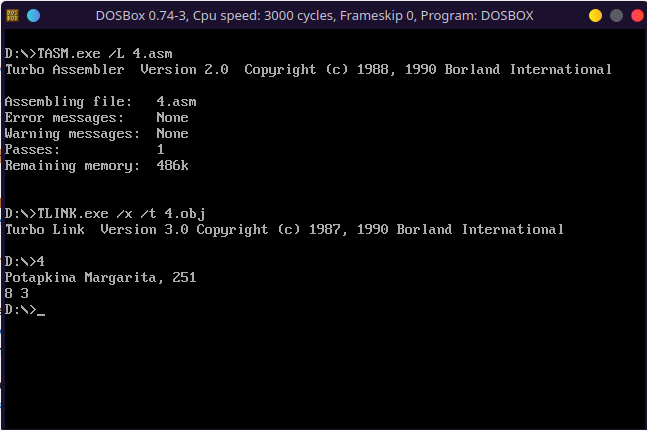
\includegraphics[scale=0.9]{4.png}
\caption {Скриншот запуска программы 1}
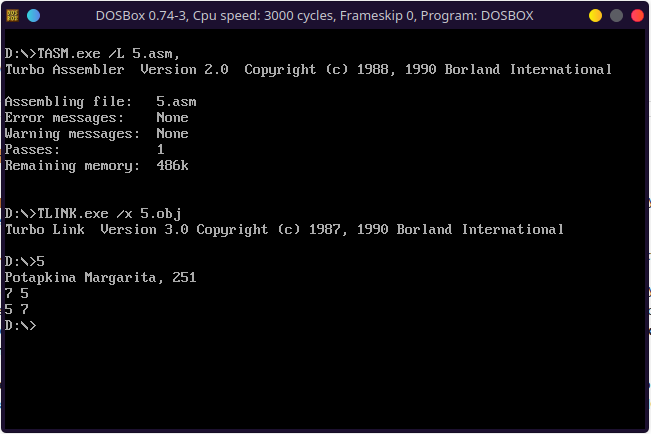
\includegraphics[scale=0.9]{5.png}
\caption {Скриншот запуска программы 2}
\end{figure}

\section{Таблицы трассировки программ с заходом внутрь вызываемых процедур (достаточно одного захода)}
\tiny
\begin{tabular}{|c|c|c|c|c|c|c|c|c|c|c|c|c|}
\hline
	Шаг & Машинный код & Команда & \multicolumn{9}{|c|}{Регистры} & Флаги \\
	& & & AX & BX & CX & DX & SP & DS & SS & CS & IP & CZSOPAID \\

\hline
	& & & 0192 & 000B & F715 & 098D & 0100 & 489D & 48B1 & 48AD & 0000 & 00000010 \\
\hline
	1 & B8AF48 & MOV AX,48AF & 48AF & 000B & F715 & 098D & 0100 & 489D & 48B1 & 48AD & 0003 & 00000010 \\
\hline
	2 & 8ED8 & MOV DS,AX & 48AF & 000B & F715 & 098D & 0100 & 48AF & 48B1 & 48AD & 0005 & 00000010 \\
\hline
	3 & B409 & MOV AH,09 & 09AF & 000B & F715 & 098D & 0100 & 48AF & 48B1 & 48AD & 0007 & 00000010 \\
\hline
	4 & BA0000 & MOV DX,0000 & 09AF & 000B & F715 & 0000 & 0100 & 48AF & 48B1 & 48AD & 000A & 00000010 \\
\hline
	5 & CD21 & INT21 & 09AF & 000B & F715 & 0000 & 0100 & 48AF & 48B1 & 48AD & 000C & 00000010 \\
\hline
	6 & B8004C & MOV AX,4C00 & 4C00 & 000B & F715 & 0000 & 0100 & 48AF & 48B1 & 48AD & 000F & 00000010 \\
\hline
	7 & CD21 & INT21 & 0192 & F560 & 0192 & F664 & 0106 & 2110 & 0192 & 0000 & 0000 & 10100011 \\
\hline
\end{tabular}


\begin{tabular}{|c|c|c|c|c|c|c|c|c|c|c|c|c|}
\hline
	Шаг & Машинный код & Команда & \multicolumn{9}{|c|}{Регистры} & Флаги \\
	& & & AX & BX & CX & DX & SP & DS & SS & CS & IP & CZSOPAID \\
\hline
	1 & B8BD48 & MOV AX,48BD & 48BD & F560 & 0192 & F664 & 0100 & 489D & 48AD & 48BF & 0003 & 00000010 \\
\hline
	2 & 8ED8 & MOV DS,AX & 48BD & F560 & 0192 & F664 & 0100 & 48BD & 48AD  & 48BF & 0005 & 00000010 \\
\hline
	3 & B409 & MOV AH,09 & 09BD & F560 & 0192 & F664 & 0100 & 48BD & 48AD & 48BF & 0007 & 00000010 \\
\hline
	4 & BA0000 & MOV DX,0000 & 09BD & F560 & 0192 & 0000 & 0100 & 48BD & 48AD & 48BF & 000A & 00000010 \\
\hline 
	5 & CD21 & INT 21 & 09BD & F560 & 0192 & 0000 & 0100 & 48BD & 48AD & 48BF & 000C & 00000010 \\
\hline
	6 & B8004C & MOV AX,4C00 & 4C00 & F560 & 0192 & 0000 & 0100 & 48BD & 48AD & 48BF & 000F & 00000010 \\
\hline
	7 & CD21 & INT21 & 0192 & F560 & 0192 & F664 & 0106 & 2110 & 0192 & 0000 & 0000 & 10100011 \\
\hline
\end{tabular}

\normalsize

\section{Ответы на контрольные вопросы}
\begin{enumerate}
\item В какой регистр надо поместить код выводимого символа? Какой код Dos"=функции используется для вывода отдельного символа на экран?

Код выводимого символа нужно поместить в регистр DL. Код используемой для вывода отдельного символа на экран Dos"=функции "--- 02h, он помещается в регистр AH.

\item Какая операция позволяет получить для цифры её код в кодовой таблице?

Если передать для отображения на экран саму цифру, то выведется символ с соответствующим ASCII"=кодом, который не будет совпадать с этой цифрой. Для получения символьной формы цифры необходимо заменить цифру ASCII"=кодом её изображения. Для этого нужно использовать команду ADD <регистр, содержащий цифру> 30h. 30h "--- ASCII"=код нуля, при прибавлении к нему цифры получится ASCII"=код этой цифры.

\item Объясните назначение процедуры. Как определяются начало и конец процедуры?

Современные программы обычно разрабатываются по модульному принципу "--- программа состоит из нескольких небольших частей, называемых подпрограммами или процедурами, и одной главной программы, которая вызывает эти процедуры на выполнение, передавая им управление процессором. После завершения работы процедуры возвращают управление главной программе и выполнение продолжается с команды, следующей за командой вызова подпрограммы. То есть процедура нужна, чтобы выполнить небольшую часть кода, причём появляется возможность переиспользовать этот код несколько раз. Описание процедуры имеет следующий синтаксис:

\input{proc.txt}

Начало процедуры определяется с помощью директивы <название процедуры> PROC, а конец "--- с помощью директивы ENDP.

\item Ваша программа состоит из главной процедуры и процедур"=подпрограмм. Каким может быть взаимное расположение главной процедуры и подпрограмм?

Процедуру можно разместить в любом месте программы, однако принято помещать её либо в конце сегмента кода, после команд завершения программы, либо в начале сегмента кода, до точки входа в программу, поскольку выполняться она должна только при обращении к ней. Также можно разместить её в отдельном кодовом сегменте.

\item Как процессор использует стек при работе с любой процедурой?

В процедуре ближнего типа (NEAR) при использовании команды вызова CALL указывается новое значение регистра IP, а в стеке сохраняется адрес возврата (IP команды, следующей после CALL). RET (команда косвенного перехода) же извлекает из стека одно слово и помещает его в регистр IP.

В процедуре дальнего типа (FAR) при вызове процедуры в стек кладутся значения регистров IP и CS, возврат же извлекает из стека 2 слова, слово из меньшего адреса помещается в регистр IP, а слово из большего "--- в CS.

\item С помощью какой команды вызывается процедура? Как меняется значение регистра SP после вызова процедуры? Приведите пример из вашей таблицы трассировки.

Процедура вызывается с помощью команды CALL <имя процедуры>. До захода в процедуру SP был равен 0100 (стек, на который изначально выделено 256 байт, был пустым), а после вызова процедуры он стал равен 00FE, т.е. уменьшился на 2. Это связано с тем, что в стек положили значение регистра IP, соответственно указатель на вершину стека уменьшился.

\item После какой команды процедуры из стека извлекается адрес возврата?
Адрес возврата из стека извлекается после команды RET, которой должна завершаться любая процедура.

\end{enumerate}
% Отобразить все источники. Даже те, на которые нет ссылок.
% \nocite{*}

% Окончание основного документа и начало приложений Каждая последующая секция
% документа будет являться приложением
\appendix
\end{document}
